\section{Interplanetary transfer}

The overall transfer is designed joining the following orbits,
that are designed according to the Restricted Two Body Problem,
with different central bodies:
\begin{enumerate}
	\item Lambert arc from Mercury to Venus (central body: Sun)
	\item gravity assist around Venus (central body: Venus)
	\item Lambert arc from Venus to Earth (central body: Sun)
	\item capture and final orbit insertion  (central body: Earth)
\end{enumerate}
The cost of the transfer is computed as the sum of:

\begin{itemize}
	\item $\Delta v_1$, required to insert the spacecraft into the departure orbit from Mercury
	\item $\Delta v_2$, required to join the hyperbolas around Venus
	\item $\Delta v_3$, required to move from the arrival hyberbola to the circular orbit
	\item $\Delta v_4$, required to move from the circular orbit to the final orbit
\end{itemize}
The overall $\Delta v$ is a function of the relative positions of the planets,
therefore it depends on the moment at which the maneuvers occur.

We define the following time instants:
\begin{itemize}
	\item $t_1$ for the departure from Mercury
	\item $t_2$ for the fly-by around Venus
	\item $t_3$ for the arrival at the Earth
\end{itemize}
Accordingly, it is possible to write $\Delta v=\Delta v(t_1,t_2,t_3)$ and to identify
the $(t_1,t_2,t_3)$ triplet for which $\Delta v$ is minimum.

In order to obtain a 2D representation,
we represent it only as a function of $t_1$ and $t_3$,
whereas $t_2 \in (t_1,t_3)$ is chosen in order to minimize the value of $\Delta v$ at fixed $(t_1,t_3)$:
$$\Delta v^*(t_1,t_3) = \min_{t_2 \in (t_1,t_3)} \Delta v(t_1,t_2,t_3)$$
This new function can be easily represented in what we call porkchop plot.

The data for the porkchop plot is evaluated using the function \textit{PorkchopData.m} (fig.~\ref{fig:flow_porkchopdata}).
As can be seen, the function is made of two nested cycles. The outermost computes $\Delta v^*(t_1,t_3)$ in the given plot range ($[t_{1,min},t_{1,max}]$,$[t_{3,min},t_{3,max}]$), while the innermost finds the minimizing $t_2$.

\begin{figure}[!htb]
\centering
\begin{tikzpicture}[auto,>=triangle 45]
    \node [startend] (start) {START};
    \node [input, below of=start, node distance=2.7cm, trapezium left angle=80, trapezium right angle=100,] (input) {Input data:\\
        gravity constants;\\
        planets' ephemerides;\\
        minimum radius for GA;\\
        final orbit parameters;\\
        $(t_1,t_3)$ pairs;\\
        time step for $t_2$};
    \node [loop, below of=input, node distance=2.7cm] (forpair) {For each $(t_1,t_3)$ pair,\\do:};
    \node [block, below of=forpair] (eph13) {Compute ephemerides for \\planet 1 at $t_1$ and planet 3 at $t_3$};
    \node [loop, below of=eph13, node distance=1.7cm] (T2split) {For each $t_2 \in (t_1,t_3)$\\(with assigned step), do:};
    \node [block, below of=T2split, node distance=1.7cm] (eph2) {Compute ephemerides for \\planet 2 at $t_2$};
    \node [block, below of=eph2] (lambert) {Design overall transfer\\using function \textit{LambertGa.m}};
    \node [block, below of=lambert] (minT2) {Keep $t_2$ that minimizes $\Delta v$};
    \node [input, below of=minT2] (return) {Return optimum $(t_2,\Delta v)$\\for each  $(t_1,t_3)$ pair};
    \node [startend, below of=return] (end) {END};

    \draw [->] (start) -- (input);
    \draw [->] (input) -- (forpair);
    \draw [->] (forpair) -- (eph13);
    \draw [->] (eph13) -- (T2split);
    \draw [->] (T2split) -- (eph2);
    \draw [->] (eph2) -- (lambert);
    \draw [->] (lambert) --  ++(5,0) |- (T2split);
    \draw [->] (T2split) -- node{end} ++(-5,0) |- (minT2);
    \draw [->] (minT2) --  ++(6,0) |- (forpair);
    \draw [->] (forpair) -- node{end} ++(-6,0) |- (return);

    \draw [->] (return) -- (end);
\end{tikzpicture}
\caption{Flow chart for function \textit{PorkchopData.m}} \label{fig:flow_porkchopdata}
\end{figure}


\begin{figure}[!htb]
\centering
\begin{tikzpicture}[auto,>=triangle 45]
    \node [startend] (start) {START};
    \node [input, below of=start, node distance=2cm] (definition) {Define problem's variables:\\
	physical quantities\\
	porkchop graph limits\\
	final orbit};
    \node [input, below of=definition, node distance=2cm] (ephemerides) {Load planets' ephemerides\\using class in Ephemerides.m};
    \node [block, below of=ephemerides] (firstporkchop) {Generate porkchop graph,\\centered in assigned $t_1$ and $t_3$};
    \node [block, below of=firstporkchop] (firstminimum) {Evaluate minimum $\Delta v$\\and corresponding $t_1$ and $t_3$};
    \node [block, below of=firstminimum] (secondporkchop) {Generate porkchop graph,\\zoomed around new $t_1$ and $t_3$};
    \node [block, below of=secondporkchop] (doagain) {Do again the last two steps};
    \node [input, below of=doagain] (output) {Print results and plot orbits};
    \node [startend, below of=output] (end) {END};

    \draw [->] (start) -- (definition);
    \draw [->] (definition) -- (ephemerides);
    \draw [->] (ephemerides) -- (firstporkchop);
    \draw [->] (firstporkchop) -- (firstminimum);
    \draw [->] (firstminimum) -- (secondporkchop);
    \draw [->] (secondporkchop) -- (doagain);
    \draw [->] (doagain) -- (output);
    \draw [->] (output) -- (end);
\end{tikzpicture}
\caption{Flow chart for script \textit{Main.m}} \label{fig:flow_main}
\end{figure}

The generation of a high-resolution porkchop plot over the whole given range would require long computation time. For this reason, at first a low-resolution plot is drawn, then it is zoomed twice in the neighbourhood of the optimum with increased resolution.
This procedure, executed by the {\it Main.m} script, is shown in fig.~\ref{fig:flow_main}.

It is now possible to identify the overall minimum:
$$\Delta v_{min}=\min_{(t_1,t_3)} \Delta v^*=\min_{(t_1,t_2,t_3)} \Delta v$$


\subsection{Lambert's problem: From Mercury to Venus and from Venus to Earth}
%The path described by the spacecraft in its motion is designed basing on the solution of the Lambert's problem through the given lambertsolver.m function.

Position and velocity vectors of the planets in the Sun-centered reference system at given time instants is obtained using ephemerides, downloaded from the JPL website (\cite{ephemerides}).

Knowing the departure and arrival planets' positions and the time of flight, the {\it lambertsolver.m} function is used to obtain the Keplerian parameters for the transfer orbit and, consequently, the departure and arrival velocity vectors ($\mathbf v_{dep}$,$\mathbf v_{arr}$).

We are required to consider null relative velocity with respect to Mercury:
$$\mathbf v_1^-=\mathbf v_{\mercury}(t_1)$$

The velocity at the starting point of the Lambert arc, given by {\it lambertsolver.m}, is:
$$\mathbf v_1^+=\mathbf v_{\mercury\rightarrow\venus,dep}$$

Therefore, the first $\Delta v_1$ is:
$$\Delta v_1 = \norm{\mathbf v_1^+ - \mathbf v_1^-}$$

\subsection{Gravity assist around Venus}

Knowing the absolute arrival and departure velocities at Venus (given by {\it lambertsolver.m}),
it is possible to compute the hyperbolic excess velocities:
\begin{align*}
\mathbf v_{\infty,\venus}^-&=\mathbf v_{\mercury\rightarrow\venus,arr}-\mathbf v_{\venus}(t_2) \\
\mathbf v_{\infty,\venus}^+&=\mathbf v_{\mercury\rightarrow\venus,dep}-\mathbf v_{\venus}(t_2)
\end{align*}

The pericenter radius that allows for the connection of the hyperbolas is found via numerical solutions.
The maneuver is considered feasible if the pericenter falls at least \SI{100}{km} above the planet's surface.

The cost of the maneuver is the difference between the pericenter velocities:

$$\Delta v_2 = \abs{v_{p,\venus,dep} - v_{p,\venus,arr}}$$

\subsection{Orbital capture around Earth}

The spacecraft reaches Earth in a hyperbolic orbit with excess velocity:
$$\mathbf v_{\infty,\oplus}^-=\mathbf v_{\venus\rightarrow\oplus,arr}-\mathbf v_{\oplus}(t_3)$$

In order to inject the spacecraft in the final orbit, an orbital maneuver has to be designed.
The arrival velocity vector can be freely shifted in order to obtain the desired pericenter radius,
in particular it is moved so as to have the same pericenter distance of the final orbit.

The two pericenters can now be connected with a circular orbit,
that belongs to the plane defined by the arrival velocity vector and the final pericenter position vector.

The cost of the maneuvers is therefore:
\begin{align*}
\Delta v_3 &= \norm{\mathbf v_{circular} - \mathbf v_{p,\oplus,arr}} \\
\Delta v_4 &= \norm{\mathbf v_{p,final} - v_{p,circular}}
\end{align*}

The computation of $\Delta v_3$ and $\Delta v_4$ is done by the function {\it Arrival.m} (fig.~\ref{fig:flow_arrival}).

\begin{figure}[!htb]
\centering
\begin{tikzpicture}[auto,>=triangle 45]
    \node [startend] (start) {START};
    \node [input, below of=start, node distance=2cm] (inputs) {Input parameters:\\
	planet's gravity parameter;\\
	arrival velocity at infinity;\\
	final orbit};
    \node [block, below of=inputs, node distance=2cm] (pericenter) {Compute final orbit pericenter's\\position and velocity};
    \node [block, below of=pericenter, node distance=1.8cm] (plane) {Build transfer orbit plane,\\containing the pericenter radius\\and the arrival velocity};
    \node [block, below of=plane, node distance=2.1cm] (firstminimum) {Shift arrival velocity vector\\in order to obtain an hyperbola\\with the same pericenter distance\\as the final orbit};
    \node [block, below of=firstminimum, node distance=2cm] (hyperbola) {Compute arrival hyperbola parameters};
    \node [block, below of=hyperbola] (circular) {Construct a circular orbit\\between the two pericenters};
    \node [input, below of=circular, node distance=2cm] (output) {Compute and output the $\Delta v$\\required to move from the \\ hyperbola to the circular orbit\\and then to the final orbit};
    \node [startend, below of=output, node distance=2cm] (end) {END};

    \draw [->] (start) -- (inputs);
    \draw [->] (inputs) -- (pericenter);
    \draw [->] (pericenter) -- (plane);
    \draw [->] (plane) -- (firstminimum);
    \draw [->] (firstminimum) -- (hyperbola);
    \draw [->] (hyperbola) -- (circular);
    \draw [->] (circular) -- (output);
    \draw [->] (output) -- (end);
\end{tikzpicture}
\caption{Flow chart for function \textit{Arrival.m}} \label{fig:flow_arrival}
\end{figure}

The computation of $\Delta v_1$ and $\Delta v_2$, and the summation of all the $\Delta v_{1,2,3,4}$ is done by the function {\it LambertGA.m} (fig.~\ref{fig:flow_lambertga}).)

%function [dVT,dV1,dV2,dV3,Rp,VIa,VFa,VIb,VFb]=LambertGA(MU0,MUGA,MU3,R1,R2,R3,V1,V2,V3,T1,T2,T3,GALimit,RpGUESS,OrbitParams_final)

\begin{figure}[!htb]
\centering
\begin{tikzpicture}[auto,>=triangle 45]
    \node [startend] (start) {START};
    \node [input, below of=start, node distance=2.7cm, trapezium left angle=80, trapezium right angle=100,] (input) {Input data:\\
        gravity constants;\\
        maneuvers' times;\\
        planets' positions and\\velocities at maneuvers' times;\\
        minimum radius for GA;\\
        final orbit parameters};
    \node [block, below of=input, node distance=2.7cm] (lambert1) {Solve first Lambert problem\\from Mercury to Venus};
    \node [block, below of=lambert1] (lambert2) {Solve second Lambert problem\\from Venus to Earth};
    \node [block, below of=lambert2] (ga) {Connect hyperbolas at Venus (GA)\\computing pericenter radius};
    \node [if, below of=ga] (isabove) {Is computed pericenter\\at least \SI{100}{km} above Venus surface?};
    \node [block, below of=isabove, node distance=3cm] (firstminimum) {Solve orbit closure at Earth};
    \node [input, below of=firstminimum, node distance=2.7cm] (return) {Return:\\
    $\Delta v$ for each maneuver;\\
    pericenter radius at GA;\\
    Lambert arcs'\\initial and final velocities};
    \node [block, right = 1cm of return, minimum width=5cm] (abort) {Abort (Return $NaN$)};
    \node [startend, below of=return, node distance=2.7cm] (end) {END};

    \draw [->] (start) -- (input);
    \draw [->] (input) -- (lambert1);
    \draw [->] (lambert1) -- (lambert2);
    \draw [->] (lambert2) -- (ga);
    \draw [->] (ga) -- (isabove);
    \draw [->] (isabove) -- node{yes} (firstminimum);
    \draw [->] (isabove.east) -- node{no}  (isabove.east -| abort.north) -- (abort);
    \draw [->] (firstminimum) -- (return);
    \draw [->] (return) -- (end);
    \draw [->] (abort) |- (end);
\end{tikzpicture}
\caption{Flow chart for function \textit{LambertGA.m}} \label{fig:flow_lambertga}
\end{figure}

\clearpage

\subsection{Results}
The plots obtained are shown below.

\begin{figure}[htp]
	\begin{subfigure}{.5\textwidth}
		\centering
		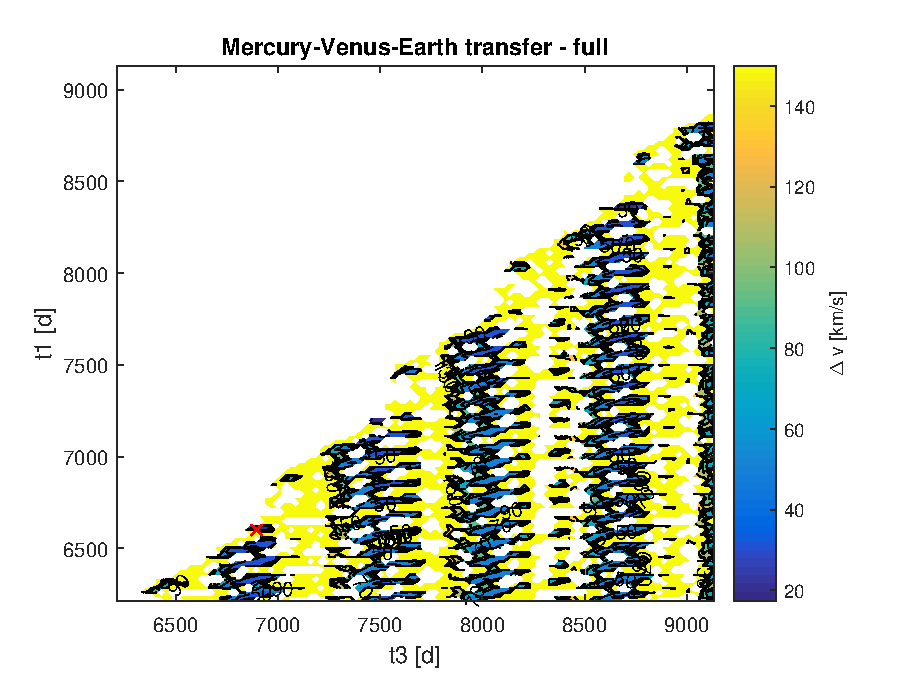
\includegraphics[width=\textwidth]{porkchop_full_contour}
	\end{subfigure}
	\begin{subfigure}{.5\textwidth}
		\centering
		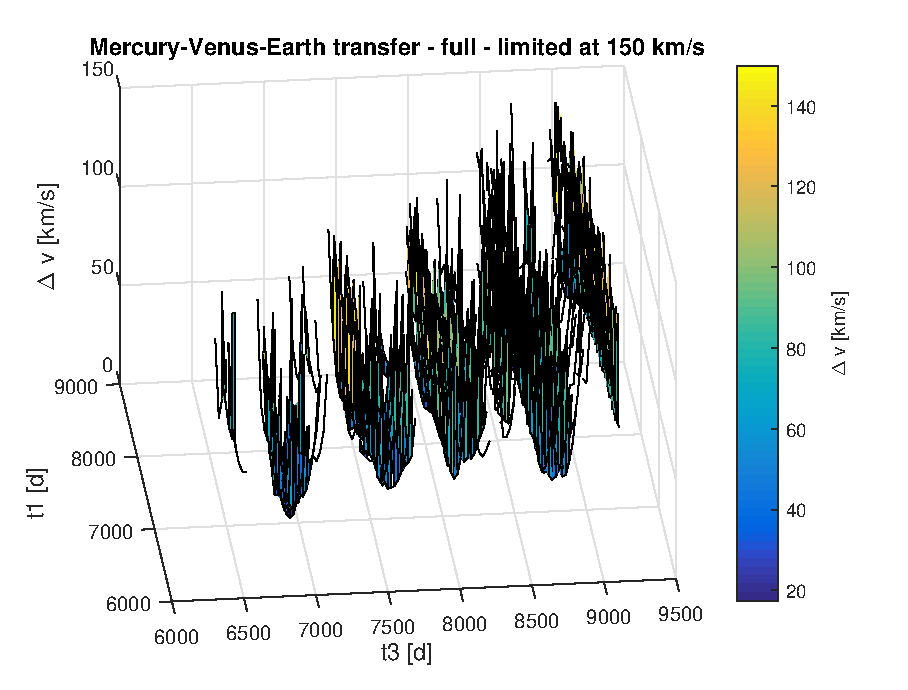
\includegraphics[width=\textwidth]{porkchop_full_surface}
	\end{subfigure}


	\begin{subfigure}{.5\textwidth}
		\centering
		\includegraphics[width=\textwidth]{porkchop_zoom1_contour}
	\end{subfigure}
	\begin{subfigure}{.5\textwidth}
		\centering
		\includegraphics[width=\textwidth]{porkchop_zoom1_surface}
	\end{subfigure}


	\begin{subfigure}{.5\textwidth}
		\centering
		\includegraphics[width=\textwidth]{porkchop_zoom2_contour}
	\end{subfigure}
	\begin{subfigure}{.5\textwidth}
		\centering
		\includegraphics[width=\textwidth]{porkchop_zoom2_surface}
	\end{subfigure}
	\caption{Porkchop plots with increasing zoom}
\end{figure}

\begin{figure}[htp]
\centering
\includegraphics[width=1.1\textwidth,trim={5cm 0 0 0},clip]{orbits_interplanetary}
\caption{Interplanetary orbits (optimum solution)}
\end{figure}
\begin{figure}[htp]
\begin{subfigure}{.5\textwidth}
\centering
\includegraphics[width=1\textwidth,trim={4.5cm 0 0 0},clip]{Venus_GA}
\caption{Gravity Assist (optimum solution)}
\end{subfigure}
\begin{subfigure}{.5\textwidth}
\centering
\includegraphics[width=1.1\textwidth,trim={5cm 0 0 0},clip]{earth_arrival}
\caption{Arrival orbital closure (optimum solution)}
\end{subfigure}
\caption{Planet-centered maneuvers detail}
\end{figure}

\clearpage
The following plots are obtained without taking into account a lower boundary for the pericenter radius during the gravity assist (Venus radius plus \SI{100}{km}).

\begin{figure}[htp]
	\begin{subfigure}{.5\textwidth}
		\centering
		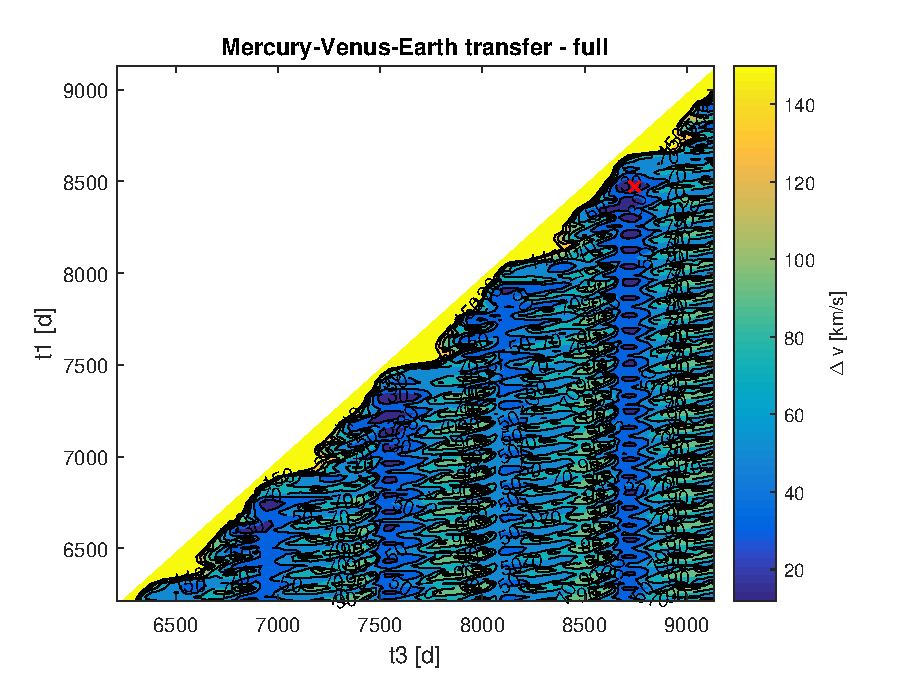
\includegraphics[width=\textwidth]{__porkchop_full_contour}
	\end{subfigure}
	\begin{subfigure}{.5\textwidth}
		\centering
		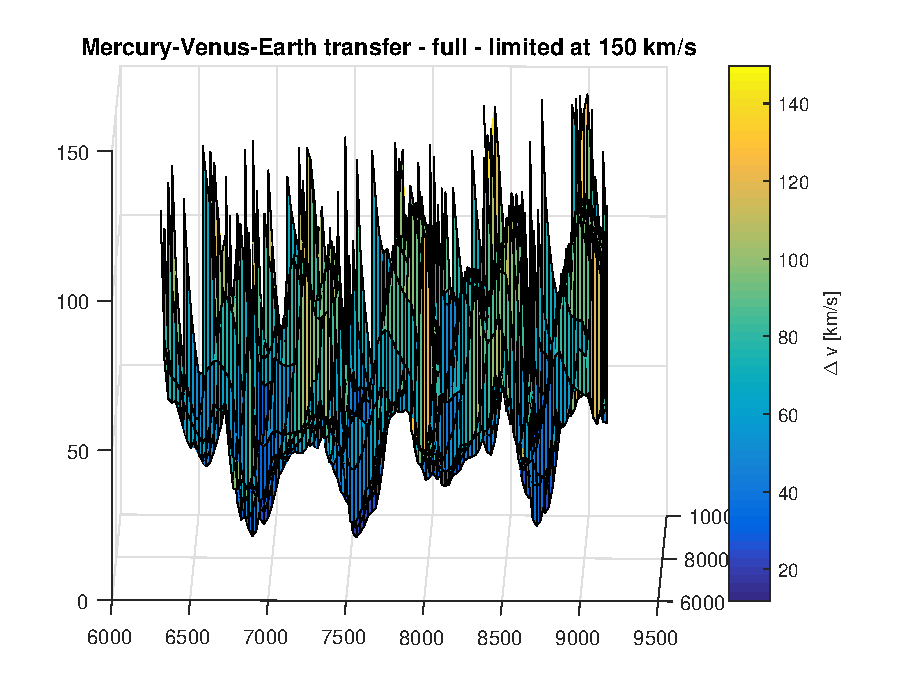
\includegraphics[width=\textwidth]{__porkchop_full_surface}
	\end{subfigure}


	\begin{subfigure}{.5\textwidth}
		\centering
		\includegraphics[width=\textwidth]{__porkchop_zoom1_contour}
	\end{subfigure}
	\begin{subfigure}{.5\textwidth}
		\centering
		\includegraphics[width=\textwidth]{__porkchop_zoom1_surface}
	\end{subfigure}


	\begin{subfigure}{.5\textwidth}
		\centering
		\includegraphics[width=\textwidth]{__porkchop_zoom2_contour}
	\end{subfigure}
	\begin{subfigure}{.5\textwidth}
		\centering
		\includegraphics[width=\textwidth]{__porkchop_zoom2_surface}
	\end{subfigure}
	\caption{Porkchop plots with increasing zoom [no limit on pericenter radius]}
\end{figure}

\begin{figure}[htp]
\centering
\includegraphics[width=1.1\textwidth,trim={5cm 0 0 0},clip]{__orbits_interplanetary}
\caption{Interplanetary orbits (optimum solution) [no limit on pericenter radius]}
\end{figure}
\begin{figure}[htp]
\begin{subfigure}{.5\textwidth}
\centering
\includegraphics[width=1\textwidth,trim={4.5cm 0 0 0},clip]{__Venus_GA}
\caption{Gravity Assist (optimum solution)}
\end{subfigure}
\begin{subfigure}{.5\textwidth}
\centering
\includegraphics[width=1.1\textwidth,trim={5cm 0 0 0},clip]{__earth_arrival}
\caption{Arrival orbital closure (optimum solution)}
\end{subfigure}
\caption{Planet-centered maneuvers detail [no limit on pericenter radius]}
\end{figure}


\clearpage
Here is reported the detailed output of the code (taking into account the lower boundary for the pericenter radius around Venus):

\noindent\rule{8cm}{0.4pt}

\verbatiminput{matlaboutput.txt}

\noindent\rule{8cm}{0.4pt}


\clearpage